\renewcommand{\theequation}{\theenumi}

\begin{theorem}\label{theorem:th1_triangle_ex}
Sum of all angles in a triangle equals $180\degree$.
\end{theorem}

\begin{enumerate}[label=\thesubsection.\arabic*.,ref=\thesubsection.\theenumi]
\numberwithin{equation}{enumi}

\item \solution  From theorem \ref{theorem:th1_triangle_ex}
\begin{align}
\angle A + \angle B + \angle C &=  180\degree
\end{align}

\item From the given information:
\begin{align}
\frac{\angle C}{6} + \frac{\angle C}{3} + \angle C &=  180\degree\\
\therefore \angle C = 120\degree \ \angle A = 20\degree \ \angle B &= 40\degree \nonumber
\end{align}

\item \begin{figure}[!h]
\centering
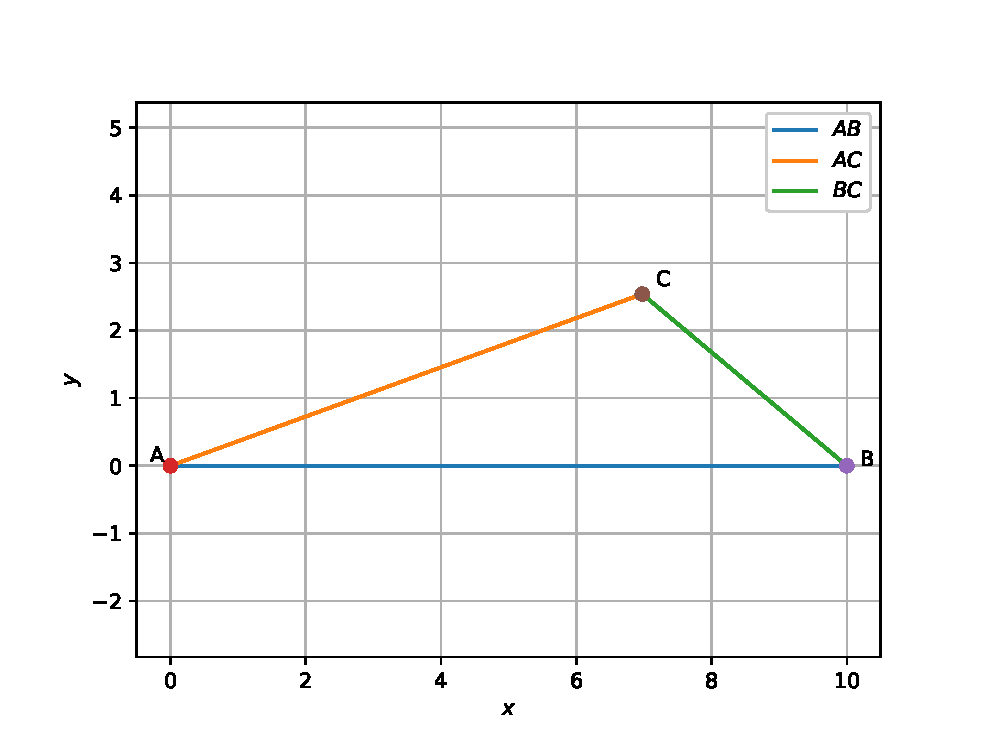
\includegraphics[width=\columnwidth]{./figs/triangle_ex/triangle_linearalg.eps}
\caption{Triangle generated using python}
\label{fig:triangle2_triangle_ex}
\end{figure} 

The  following Python code generates Fig. \ref{fig:triangle2_triangle_ex}

\begin{lstlisting}
codes/triangle_ex/triangle_linearalg.py
\end{lstlisting}

\end{enumerate}

\pagebreak
